\documentclass[utf8]{beamer}
\usefonttheme[onlymath]{serif}

\mode<presentation>
{
  \usetheme{Warsaw}
  \setbeamercovered{transparent}
}

\usepackage[utf8]{inputenc}
\usepackage[T2A]{fontenc}
\usepackage[russian]{babel}

\usepackage{mathtools, amssymb, bm}
%% \usepackage{IEEEtrantools}

\usepackage{graphicx}
% set up graphicx to use custom path to graphs
\graphicspath{{../graphs/}}

\usepackage{tabu}
%% \usepackage{footnote}

\usepackage[norelsize,ruled,vlined]{algorithm2e}

\title[Обработка множеств логических закономерностей]{
  \small{
    Обработка множеств логических закономерностей с помощью
    дисперсионного критерия
  }
}

\subtitle{Выпускная квалификационная работа} % (optional)

\author[Рязанов~В.\,В., Лисяной~А.\,Е.]{
  \small{%
    \emph{Выполнил:}~Лисяной~А.\,Е. \\%
    \emph{Руководитель:}~д.ф.-м.н.,~проф.~Рязанов~В.\,В. \\%
  }
}

\institute[МГУ им. М.\,В.~Ломоносова]
{
  Факультет Вычислительной Математики и Кибернетики \\
  Кафедра Математических Методов Прогнозирования \\
  МГУ им. М.\,В.~Ломоносова
}

\date[\today]{\today}

\DeclareMathOperator*{\argmin}{arg\,min}
\DeclareMathOperator*{\argmax}{arg\,max}

\begin{document}

\begin{frame}
  \titlepage
\end{frame}

\begin{frame}{Задача классификации}
  \begin{block}{Определение задачи классификации}
    Пусть имеется пространство объектов \(X\) и
    конечное множество имен классов \(Y = \left\{1, \dots,
    M\right\}\). Пусть также имеется \emph{обучающая выборка} \(X^{l} =
    (x_i, y_i)_{i = 1}^{l}\), в которой для каждого объекта \(x_i\)
    известен его класс \(y_i \in Y\).  Для восстановления целевой
    зависимости \(y^{*}(x_i) = y_i\) построим алгоритм классификации
    \(a\colon X \rightarrow Y\), аппроксимирующий \(y^{*}\) на всём
    пространстве объектов \(X\).
  \end{block}
    \begin{block}{Алгоритмы решения задачи классификации}
    \begin{itemize}
    \item Метод логистической регрессии
    \item Метод опорных векторов
    \item Решающие деревья
    \item Нейронные сети
    \item Логические алгоритмы классификации
    \end{itemize}
  \end{block}
\end{frame}

\begin{frame}{Методы поиска логических закономерностей}
  \begin{block}{Определение логической закономерности}
    Пусть каждый объект выборки \(x\in X^l\) имеет размерность \(D\) и
    пусть \(\Omega\subseteq\left\{1, 2, \dots, D\right\}\). Предикат
    \[
    \varphi(x) = P^{\Omega, \bm{c_1}, \bm{c_2}}(x) =
    \bigwedge_{j\in\Omega}P^{c_1^j, c_2^j}(f_j(x))
    \]
    называется логической закономерностью класса \(K\), если выполнено:
    \begin{enumerate}
    \item \(\exists x\in K\colon \varphi(x) = 1\)
    \item \(\forall x\not\in K\colon \varphi(x) = 0\)
    \item \(\varphi(x)\) максимизирует некоторый критерий качества
      предиката \(\Phi\).
    \end{enumerate}
  \end{block}
\end{frame}

\begin{frame}{Обработка множества логических закономерностей}
  Построенное множество логических закономерностей:
  \begin{itemize}
  \item может содержать большое количество правил
  \item может содержать похожие правила
  \end{itemize}
  Это приводит к тому, что:
  \begin{itemize}
  \item логические закономерности сложно интерпретировать
  \item по похожим правилам плохо проводить классификацию
  \end{itemize}
  \begin{block}{Задача обработки множества логических закономерностей}
    \begin{itemize}
      \item По исходному множеству логических закономерностей
        построить множество меньшей мощности, что должно упростить
        пользователю задачу интерпретации полученных правил.
      \item Построенное множество логических закономерностей меньшей
        мощности должно иметь качество классификации, сравнимое с
        исходным множеством.
      \end{itemize}
  \end{block}
\end{frame}

\begin{frame}{Обработка множества логических закономерностей}
  \begin{enumerate}
  \item Для каждого из \(t\) правил cоставить признаковое описание
  \item Кластеризовать на \(k\leq t\) кластеров, найти их центры
  \item По центрам кластеров построить \(k\) новых правил
  \end{enumerate}
    \begin{table}[!htbp]
      \begin{tabu}{X[1.2] X[2] X[2.8] X}
        Выборка & Всего объектов & Объекты по классам & Признаки\\\hline
        Iris & 150 & 50/50/50 & 4   \\
        Wine & 178 & 59/71/48 & 13  \\
        Climate & 540 & 46/494   & 11  \\
        Ionosphere & 351 & 126/255  & 34  \\
      \end{tabu}
      \caption{Сводная таблица по использованным данным}
    \end{table}
\end{frame}

\begin{frame}
  \centering
  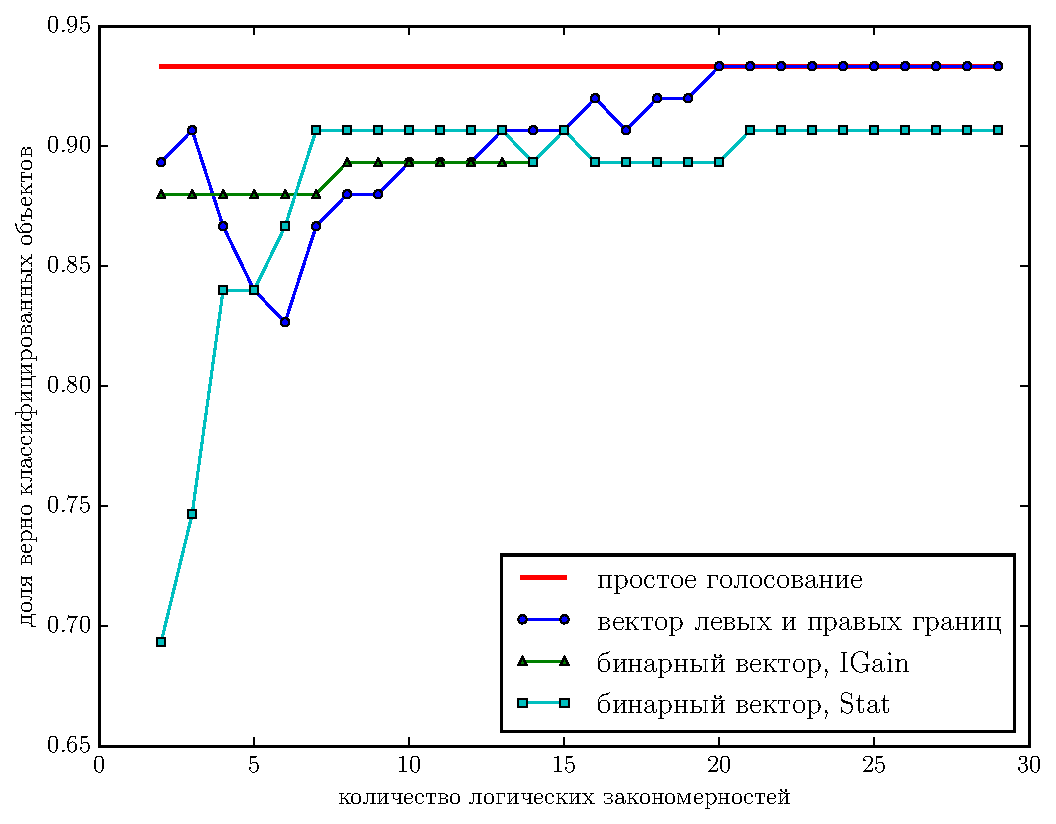
\includegraphics[width=0.8\textwidth,keepaspectratio]{iris}
  \\ Выборка Iris. Классификация методом простого голосования
\end{frame}

\begin{frame}
  \centering
  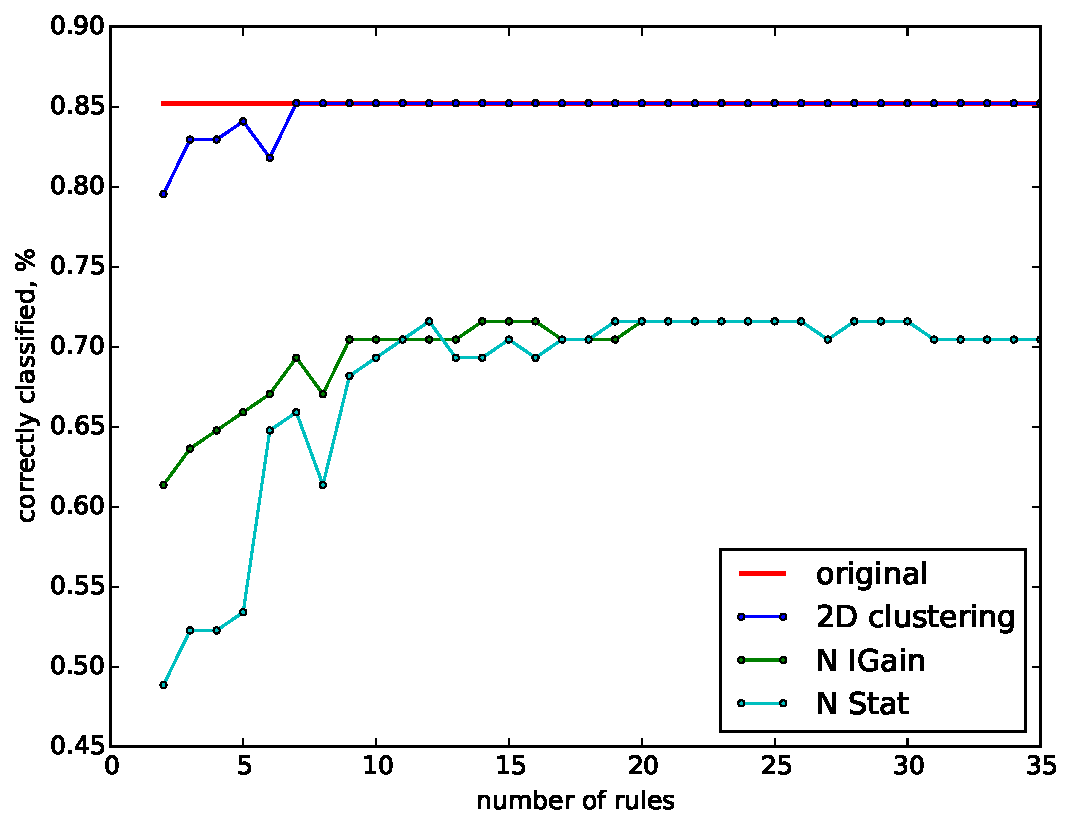
\includegraphics[width=0.8\textwidth,keepaspectratio]{wine}
  \\ Выборка Wine. Классификация методом простого голосования
\end{frame}

\begin{frame}{Список результатов}
  \begin{itemize}
    \item Реализован метод обработки множеств логических
      закономерностей с помощью кластеризации на основе дисперсионного
      критерия.
    \item Проведено сравнение метода обработки, использующего вектор
      левых и правых границ, и метода обработки, использующего
      бинаризованное описание логических закономерностей.
    \item Экспериментально показано, что удается получить обработанное
      множество логических закономерностей с меньшим числом элементов
      и сравнимым с исходным множеством качеством классификации.
  \end{itemize}
\end{frame}


\end{document}
